% -*- TeX-master: "main"; fill-column: 72 -*-

\newpage
\section{HARMONY: proposed extensions 2018}

\begin{quote}
 \textbf{\Large The contents of this section are unofficial and are formulated here in order to make efficient use of time at HARMONY 2018.}
\end{quote}

\subsection{The extended \class{SBase} class}
\label{sbase-class-kv}

The \SBML \SBase class is extended by a \token{listOfKeyValues} of which it may contain at most one.
%
\begin{figure}[ht]
  \centering
  % Requires \usepackage{graphicx}
  %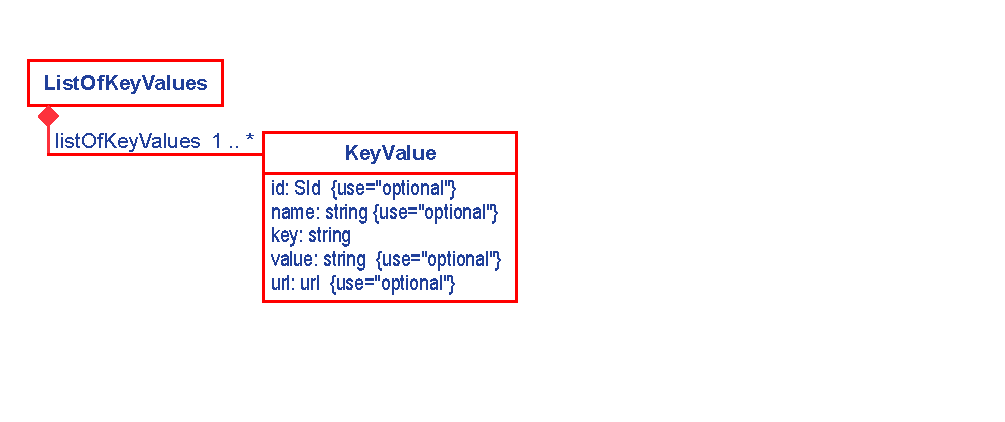
\includegraphics[width=6cm]{images/fbc_v3_uml_keyvalue.pdf}\\
  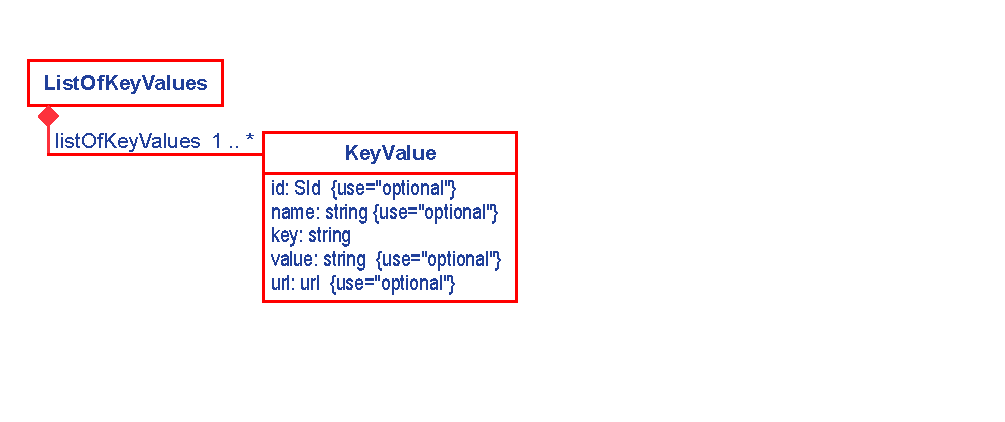
\includegraphics[width=0.6\textwidth]{images/fbc_v3_uml_keyvalue.pdf}\\
  \caption{A UML representation of the \SBML \SBase class extended in
  the \FBCPackage by the \ListOfKeyValues. See \ref{conventions} for conventions related to this
  figure.}
  \label{fig:fbc_v3_uml_keyvalue}
\end{figure}


\subsection{The extended \class{Model} class}
\label{model-class-kv}
%\label{listoffluxbounds-class}

The \SBML \Model class is extended by a \token{listOfAdditionalConstraints} of which it may contain at most one.
%
\begin{figure}[ht]
  \centering
  % Requires \usepackage{graphicx}
  %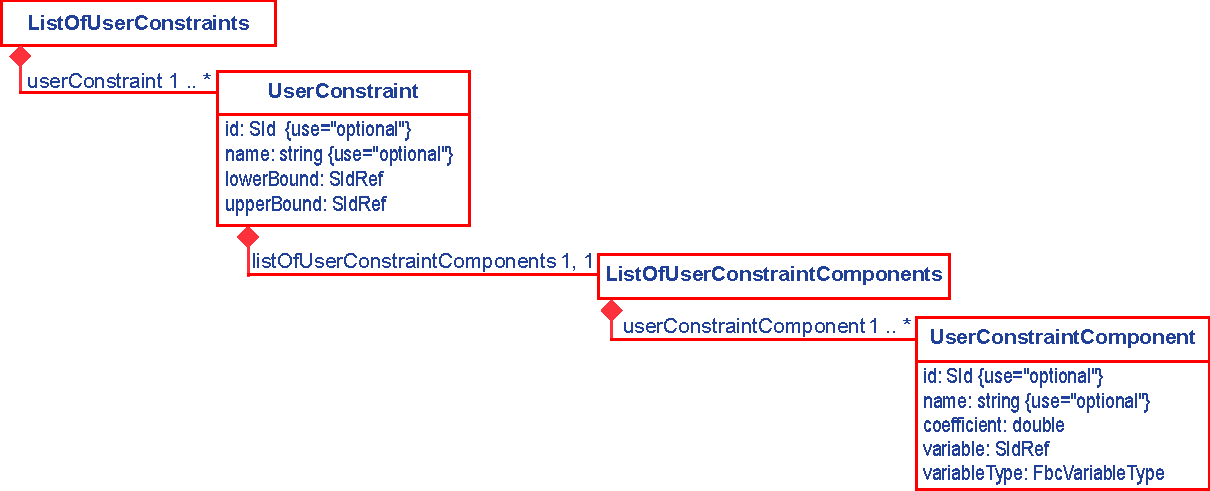
\includegraphics[width=6cm]{images/fbc_v3_uml_userconstraint.pdf}\\
  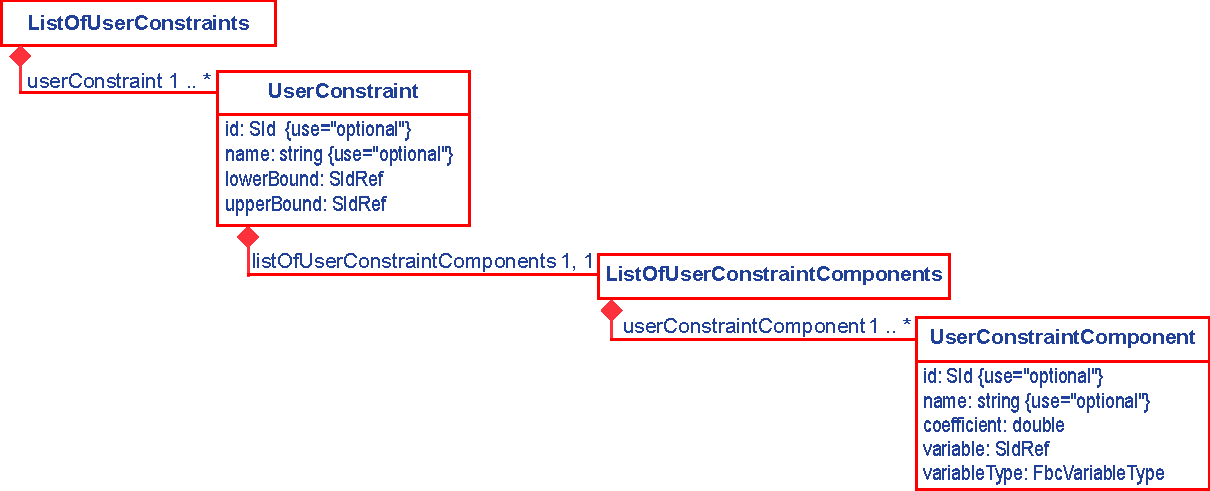
\includegraphics[width=\textwidth]{images/fbc_v3_uml_userconstraint.pdf}\\
  \caption{A UML representation of the \SBML \Model class extended in
  the \FBCPackage by the\ListOfUserConstraints. See \ref{conventions} for conventions related to this
  figure.}
  \label{fig:fbc_v3_uml_user_constraints}
\end{figure}


\subsubsection{Type \primtypeNC{FbcFOVariableType}}
\label{primtype-fbcfluxobjectivevariabletype}

The \FBCPackage defines a new enumerated type \primtype{FbcFOVariableType} which
represents the index of a variable that occurs in the objective function. It can have one
of the following two values \val{linear} or \val{quadratic}.

\subsubsection{Type \primtypeNC{FbcUCCVariableType}}
\label{primtype-fbcuserconstraintvariabletype}

The \FBCPackage defines a new enumerated type \primtype{FbcUCCVariableType} which
represents the index of a variable that occurs in a user defined constraint. It can have one
of the following two values \val{linear} or \val{quadratic}.

\subsection{The \FBC \class{FluxObjective} class}

\paragraph{The \token{variableType} attribute}
The required \token{variableType} attribute contains a \primtype{FbcFOVariableType} that
represents the index of a variable that occurs in a \FluxObjective. It can have one
of the following two values \val{linear} or \val{quadratic}.
%
\begin{figure}[ht]
  \centering
  % Requires \usepackage{graphicx}
  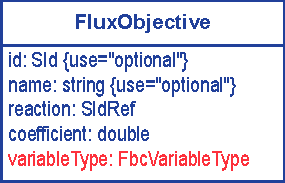
\includegraphics[width=6cm]{images/fbc_v3_uml_fobj.pdf}\\
  \caption{A UML representation of the \FBCPackage \FluxObjective class. For a complete description see \ref{fig:fbc_uml} as well as \ref{conventions} for conventions related to this figure.}
  \label{fig:fbc_uml_userconstraint}
\end{figure}

\subsubsection{The \FBC \class{listOfUserConstraints}}
\label{listofuserconstraints-class}

As shown in \ref{fig:fbc_v3_uml_user_constraints} the \ListOfUserConstraints is derived from \SBase
and inherits the attributes \token{metaid} and \token{sboTerm}, as well as
the subcomponents for \Annotation and \Notes. The
\ListOfUserConstraints must contain at least one \UserConstraint (defined in
\ref{userconstraint-class}).

\subsection{The \FBC \class{UserConstraint} class}
\label{userconstraint-class}

The \FBC \UserConstraint class is derived from \SBML \SBase and inherits
\token{metaid} and \token{sboTerm}, as well as the subcomponents for
\Annotation and \Notes. It's purpose is to define non-stoichiometric constraints, i.e., constraints that are not implicitly defined by the reaction network. The \UserConstraint contains a linear combination of \UserConstraintComponent's contained in a \ListOfUserConstraintComponents.

\paragraph{The \token{id} and \token{name} attributes}
An \UserConstraint has an optional \token{id} of type
\primtype{SId} and an optional attribute \token{name} of type \primtype{string}.

\paragraph{The \token{leftHandSide} attribute}
The required \token{leftHandSide} attribute contains an \primtype{SIdRef} that references a \Parameter which contains the lower boundary value of the \UserConstraint.

\paragraph{The \token{rightHandSide} attribute}
The required \token{rightHandSide} attribute contains an \primtype{SIdRef} that references a \Parameter which contains the upper boundary value of the \UserConstraint.

\paragraph{The \token{listOfUserConstraintComponents} element}
\label{listofuserconstraintcomponents-class}

The element \token{listOfUserConstraintComponents} which contains a
\ListOfUserConstraintComponents is derived from and functions like a typical \SBML
\textsf{\textbf{ListOf\rule{0.15in}{0.5pt}}} class with the restriction that it
must contain one or more elements of type \UserConstraintComponent (see \ref{userconstraintcomponent-class}).
This implies that if a \UserConstraint is defined there should be at least
one \UserConstraintComponent contained in a \ListOfUserConstraintComponents.

%\begin{figure}[ht]
%  \centering
%  % Requires \usepackage{graphicx}
%  %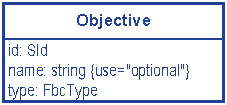
\includegraphics[width=5cm]{images/v2harmony_fbc_objective.pdf}\\
%  \caption{A UML representation of the \FBCPackage \UserConstraint class. For a complete description see \ref{fig:fbc_uml} as well as \ref{conventions} for conventions related to this figure.}
%  \label{fig:fbc_uml_userconstraint}
%\end{figure}

\subsection{The \FBC \class{UserConstraintComponent} class}
\label{userconstraintcomponent-class}

The \FBC \UserConstraintComponent class is derived from \SBML \SBase and inherits
\token{metaid} and \token{sboTerm}, as well as the subcomponents for
\Annotation and \Notes. The \UserConstraintComponent class is a relatively simple container for a variable type specifier, a variable weighted by a signed coefficient.

\paragraph{The \token{id} and \token{name} attributes}
An \UserConstraintComponent has an optional \token{id} of type \primtype{SId} and an optional attribute \token{name} of type \primtype{string}.

\paragraph{The \token{coefficient} attribute}
The required \token{coefficient} attribute contains an \primtype{SIdRef} that is restricted to reference only a \Parameter which then holds the coefficient value (\newtxt{in strict mode should we disallow this parameter to be NaN and +-inf?}).

\paragraph{The \token{variable} attribute}
The required \token{variable} attribute contains an \primtype{SIdRef} that is restricted to reference the \primtype{SId} of either a \Reaction or (\newtxt{non-constant?}) \Parameter.

\paragraph{The \token{variableType} attribute}
The required \token{variableType} attribute contains a \primtype{FbcUCCVariableType} that indicates whether a variable should be considered as `linear' or `quadratic'.

\subsubsection{The \FBC \class{listOfKeyValues}}
\label{listofkeyvalues-class}
As shown in \ref{fig:fbc_v3_uml_keyvalue} the \ListOfKeyValues extends \SBase and defines the \token{listOfKeyValues}. It \newtxt{does not} inherit the
attributes \token{metaid} and \token{sboTerm}, as well as the subcomponents for \Annotation and \Notes. The \ListOfKeyValues contains \KeyValue's (defined in \ref{keyvalue-class}).

\subsection{The \FBC \class{KeyValue} class}
\label{keyvalue-class}

The \FBC \KeyValue class is not derived from \SBML \SBase and \newtxt{does not} inherit
\token{metaid} and \token{sboTerm}, as well as the subcomponents for
\Annotation and \Notes. It's purpose is to define a tuple containing a
structured key--value pair.

\paragraph{The \token{id} and \token{name} attributes}
An \UserConstraint has an optional \token{id} of type
\primtype{SId} and an optional attribute \token{name} of type \primtype{string}.

\paragraph{The \token{key} attribute}
The \token{key} is the only mandatory component of the \KeyValue and is of type \primtype{string}.

\paragraph{The \token{url} attribute}
The optional attribute \token{url} is of type \primtype{url} and is designed to point to a resource that defines the aforementioned \token{key} attribute.

\paragraph{The \token{value} attribute}
The optional \token{value} attribute is of \primtype{string} and contains the value referred to by the \token{key} and optionally, the \token{url}. 